% Chapter Template

\chapter{Desarrollo}

\label{Chapter4} % Change X to a consecutive number; for referencing this chapter elsewhere, use \ref{ChapterX}

Una vez presentado el contexto, los objetivos, así como las herramientas empleadas y los fundamentos teóricos, en este capítulo se detallará la solución software final desarrollada. Primero se presenta el diseño global utilizado y después se analizará en detalle el componente en cuestión realizado con una visión profunda del desarrollo por bloques y su funcionamiento.


%-----------------------------------
%	SECTION Diseño
%-----------------------------------
\section{Diseño}

El trabajo se basa principalmente en dos componentes; un componente de JDeRobot (\textbf{OpenniServer}) que funciona como driver del sensor y proporciona las imágenes obtenidas por éste y el componente realizado (\textbf{realRTEstimator}) que se encargará, una vez recogidas las imágenes, de toda la lógica restante.

El objetivo del componente, como ya se ha comentado, consiste en analizar en tiempo real la posición y movimiento del sensor, por lo que el componente deberá dar una estimación en todo momento.

En la Figura~\ref{fig:diagram1} se puede apreciar el diagrama global de funcionamiento del componente desarrollado y su conexión con otros componentes para los diferentes datos de entrada.

\begin{figure}[th]
\centering
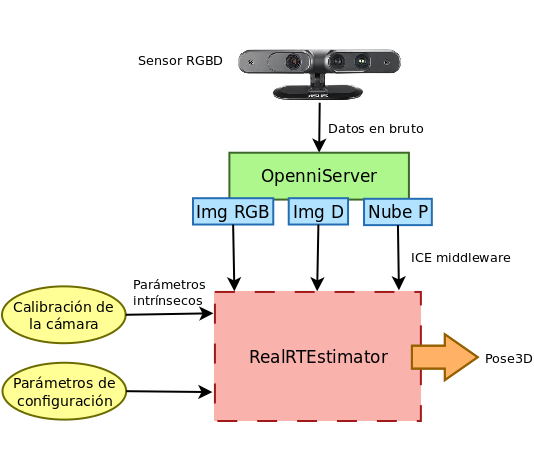
\includegraphics[scale=0.5]{Figures/diagram1.png}
\decoRule
\caption[Diagram1]{Esquema global de funcionamiento.}
\label{fig:diagram1}
\end{figure}

OpenniServer se encarga de preparar y enviar las imágenes del sensor. El componente recoge las imágenes a través de ICE y éste es el encargado de procesarlas. También recibe los datos de los parámetros intrínsecos de la cámara así como algunos parámetros de configuración, como pueden ser la activación/desactivación de la interfaz de usuario o algunos parámetros configurables de algunos de los algoritmos internos. A su salida entrega una matriz RT que describe la posición y orientación absolutas en ese preciso instante de tiempo. 

Respecto al funcionamiento interno del componente se puede ver a grandes rasgos el diagrama en la Figura~\ref{fig:diagram2}. Se observa el diseño implementado así como sus bloques funcionales:

\begin{figure}[!ht]
\centering
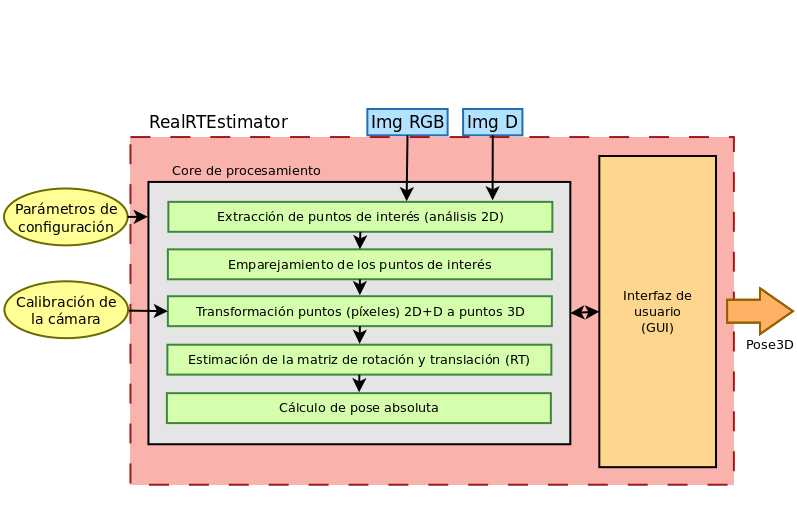
\includegraphics[scale=0.36]{Figures/diagram2.png}
\decoRule
\caption[Diagram2]{Diagrama del componente RealRTEstimator.}
\label{fig:diagram2}
\end{figure}

\begin{itemize}
\item Extración de puntos de interés (análisis 2D) del fotograma actual.

\item Emparejamientos de puntos de interés en t con respecto a los puntos extraídos en el instante anterior (t-1).

\item Transformación de puntos (píxeles) en 2D más imagen de profundidad a nube de puntos en 3D.

\item Cálculo de movimiento. Es decir, estimación de la matriz de rotación y translación (Matriz RT).

\item Calculo de pose 3D absoluta.

\end{itemize}

En las siguientes secciones desglosaremos el funcionamiento de estos diferentes bloques funcionales.

%-----------------------------------
%	SECTION Extracción de características de una imágen
%-----------------------------------
\section{Análisis 2D}

Extracción de características de una imágen

\subsection{Puntos de interés}

%-----------------------------------
%	SECTION Emparejamiento (\textit{matching})
%-----------------------------------
\section{Emparejamiento (\textit{matching})}

%-----------------------------------
%	SUBSECTION Cálculo de movimiento
%-----------------------------------
\section{Cálculo de movimiento}

\subsection{Matriz RT}

%-----------------------------------
%	SECTION Interfaz gráfica
%-----------------------------------
\section{Interfaz gráfica}